\chapter{Finite element method: formulation}

\disclaimer

\section{Introduction}
In this lecture, we develop finite element approximations of variational problems.  Specifically, we introduce a triangulation of the domain $\Omega$, construct an approximation space $\calV_h \subset \calV$, formulate a discrete problem, and then discuss the well-posedness of the finite element problem.

\section{Triangulation}
We first introduce a \emph{triangulation} of $\Omega \subset \RR^d$.  A triangulation
\begin{equation*}
  \calT_h \equiv \{ K_i \}_{i=1}^{n_e}
\end{equation*}
is a set of non-overlapping elements $K_1, \dots, K_{n_e}$ such that the union of the closure of the elements covers the domain:
\begin{align*}
  K_i \cap K_j &= \emptyset,  \quad i \neq j \\
  \cup_{i=1}^{n_e} \overline K_i &= \overline \Omega.
\end{align*}
(We consider the closure of the elements because we consider each element to be open.) An example of a triangulation is shown in Figure~\ref{fig:fe_mesh_p1}. The triangulation comprises $n_e = 9$ triangular elements $\{K_i\}_{i=1}^{n_e}$, which are delineated by $n_v = 9$ vertices $\{z_i\}_{i=1}^{n_v}$. For each element $K_i$, we define the \emph{diameter}
\begin{equation*}
  h_{K_i} \equiv \text{diam}(K_i).
\end{equation*}
The diameter of $K_i$ is the supremum of the distances between pairs of points in $K^i$,
\begin{equation*}
  \text{diam}(K_i) = \sup_{x,y \in K_i} \| x - y \|_2;
\end{equation*}
the diameter for a triangle $K_i$ is the length of the longest edge. (We take the supremum because each element is open.) The subscript $h$ of the triangulation $\calT_h$ signifies the maximum diameter of the elements in the triangulation,
\begin{equation*}
  h \equiv \max_{i = 1,\dots,n_e} h_{K_i}.
\end{equation*}
  Intuitively (and as we will see more formally), the finite element spaces associated with a sequence of triangulations get richer as $h$ decreases.  In general, a triangulation comprises line segments in one dimension, triangles or quadrilaterals in two dimension, and tetrahedrons or hexahedrons in three dimensions.


\begin{figure}
  \centering
  \subfigure[mesh]{
    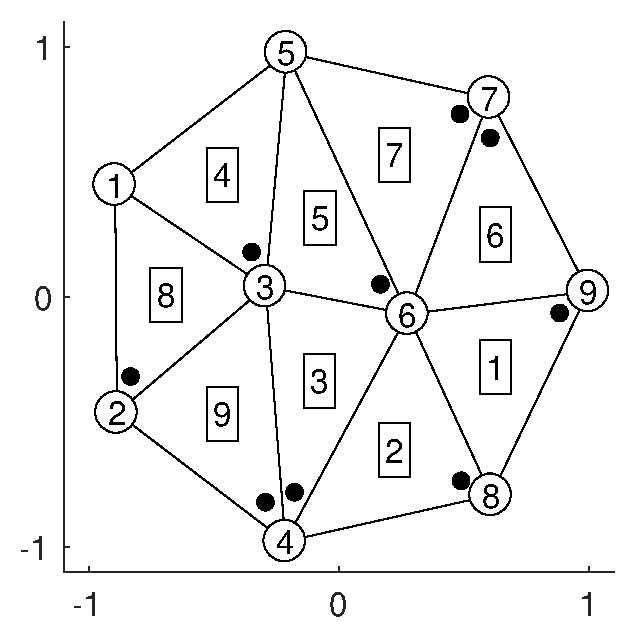
\includegraphics[width=0.4\textwidth]{fe_mesh_p1}
  }
  \caption{Triangulation.}
  \label{fig:fe_mesh_p1}
\end{figure}

While mathematically a triangulation is simply a collection of non-overlapping elements that cover the domain, we need a convenient means to represent the triangulation on a computer.  One approach is to store tables of \emph{node coordinates} and \emph{element-node connectivities}.  Tables~\ref{tb:fe_mesh_p1_coord} and \ref{tb:fe_mesh_p1_tri} are respectively the coordinate and connectivity tables associated with the triangulation shown in Figure~\ref{fig:fe_mesh_p1}. The connectivity table indicates that, for instance, the element $K_5$ is delineated by the nodes $z_6$, $z_5$, and $z_3$; the coordinate table then indicates that the coordinates of these three nodes are $z_6 = (0.28,-0.07)$, $z_5 = (-0.21,0.98)$, and $z_3 = (-0.29,0.04)$. By convention, we order the nodes of the triangles in the counter-clockwise manner. The coordinate and connectivity tables together provide a complete geometric description of all elements.  Note that, in Figure~\ref{fig:fe_mesh_p1}, for each triangle, we indicate the first of the three nodes that delineate the triangle by a dot ($\bullet$); with this convention we have identical information presented in Figure~\ref{fig:fe_mesh_p1} in a visual form and Tables~\ref{tb:fe_mesh_p1_coord} and \ref{tb:fe_mesh_p1_tri} in an array form.

\begin{table}
  \centering
  \caption{Node coordinate and connectivity table for mesh shown in Figure~\ref{fig:fe_mesh_p1}.  \label{tb:fe_mesh_p1}}
    \subfigure[coordinates]{
      \label{tb:fe_mesh_p1_coord}
    \begin{tabular}{c|cc}
      node & $x_1$ & $x_2$ \\
      \hline
      $1$ & $-0.89$ & $\hphantom{-}0.45$ \\ 
      $2$ & $-0.89$ & $-0.46$ \\ 
      $3$ & $-0.29$ & $\hphantom{-}0.04$ \\ 
      $4$ & $-0.21$ & $-0.98$ \\ 
      $5$ & $-0.21$ & $\hphantom{-}0.98$ \\ 
      $6$ & $\hphantom{-}0.28$ & $-0.07$ \\ 
      $7$ & $\hphantom{-}0.60$ & $\hphantom{-}0.80$ \\ 
      $8$ & $\hphantom{-}0.61$ & $-0.79$ \\ 
      $9$ & $\hphantom{-}1.00$ & $\hphantom{-}0.02$ \\ 
    \end{tabular}
  }
    \subfigure[connectivity]{
          \label{tb:fe_mesh_p1_tri}
    \begin{tabular}{c|ccc}
      element & node 1 & node 2 & node 3 \\
      \hline
      $1$ & $9$ & $6$ & $8$ \\ 
      $2$ & $8$ & $6$ & $4$ \\ 
      $3$ & $4$ & $6$ & $3$ \\ 
      $4$ & $3$ & $5$ & $1$ \\ 
      $5$ & $6$ & $5$ & $3$ \\ 
      $6$ & $7$ & $6$ & $9$ \\ 
      $7$ & $7$ & $5$ & $6$ \\ 
      $8$ & $2$ & $3$ & $1$ \\ 
      $9$ & $4$ & $3$ & $2$ \\ 
    \end{tabular}
    }
\end{table}

The task of generating a triangulation for a given domain is called \emph{mesh generation} and a software that carries out the task is called a \emph{mesh generator} or \emph{mesher}.  Mesh generation is a non-trivial task.  In fact, the development of algorithms that can robustly and automatically generate high-quality triangulation for complex geometries in three dimensions is an area of ongoing research.  Nevertheless, because mesh generation is essential for any finite element discretization, there are many commercial and open-source meshers.  Here we name a few user-friendly, open-source meshers:
\begin{itemize}
\item \texttt{triangle}. A robust two-dimensional mesher written in C that generates meshes with a guaranteed quality certificate in terms of the minimal angle.
\item \texttt{tetgen}. A popular three-dimensional mesher written in C.
\item \texttt{distmesh}.  A user-friendly mesher written in \textsc{Matlab} for implicit domain geometries represented by level sets. 
\end{itemize}
The mesh shown in Figure~\ref{fig:fe_mesh_p1} was in fact generated by \texttt{distmesh}.  We will extensively use \texttt{distmesh} to generate meshes in this course as it is implemented in \textsc{Matlab} and is easy to use.


\section{Approximation spaces}
We now introduce \emph{approximation spaces} for $\calV$.  An approximation space is a finite-dimensional subspace space of $\calV$ with which we can approximate functions in $\calV$. For concreteness, we consider a piecewise linear approximation space for $\calV \equiv H^1(\Omega)$ associated with the triangulation $\calT_h$,
\begin{equation}
  \calV_h \equiv \{ v \in \calV \equiv H^1(\Omega) \ | \ v|_K \in \PP^1(K), \ \forall K \in \calT_h \};
  \label{eq:fe_lin_Vh}
\end{equation}
here $\PP^1(K)$ is the space of linear polynomials over $K$. We note the two requirements: $v \in \calV_h$ must belong to $\calV \equiv H^1(\Omega)$;  $v$ restricted to any element $K \in \calT_h$, $v|_K$, must be a linear polynomial. Figure~\ref{fig:fe_fun_p1} shows an example of a function in a linear ($\PP^1$) finite element space, associated with the mesh shown in Figure~\ref{fig:fe_mesh_p1}.

%% \begin{equation*}
%%   \calV_h \equiv \{ v \in \calV \equiv H^1(\Omega) \ | \ v|_K \in \PP^p(K), \ K \in \calT_h \},
%%   \label{eq:fe_Vh}
%% \end{equation*}
%where $\PP^p(K)$ is the space of polynomials of degree at most $p$ over $K$.


\begin{figure}
  \centering
  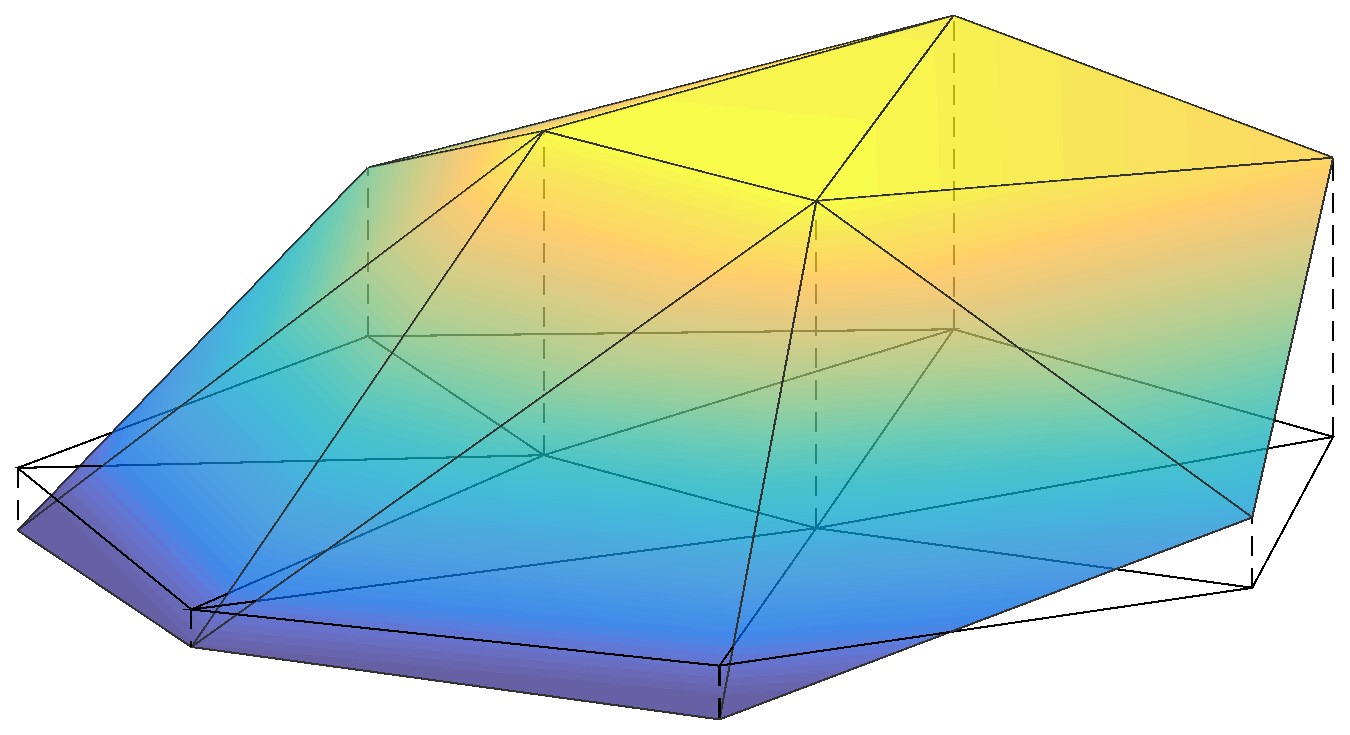
\includegraphics[width=0.45\textwidth]{fe_fun_p1}
  \caption{A function in a linear finite element space.}
  \label{fig:fe_fun_p1}
\end{figure}

We note that the condition $\calV_h \subset H^1(\Omega)$ means that the weak derivative of functions must be square integrable (in the Lebesgue sense); for piecewise polynomials, the condition is satisfied if and only if the function is continuous.  To see this, we observe the following.  If a function is continuous and piecewise polynomial, the weak first derivative is a (potentially discontinuous) piecewise polynomial and hence is square integrable; the function hence is in $H^1(\Omega)$.  If a function is not continuous across element interfaces, then the weak first derivative generates delta distributions at the interfaces and hence is not in $L^2(\Omega)$; recall for instance a concrete example for a Heaviside-like function in Section~\ref{sec:posnd_sobolev}. Hence, for a piecewise polynomial function, the continuity is a necessary and sufficient condition for the function to be in $H^1(\Omega)$. 

We now need a convenient means to describe functions in $\calV_h$ given by~\eqref{eq:fe_lin_Vh}, such as the one shown in Figure~\ref{fig:fe_fun_p1}.  Specifically, we need to pick \emph{global degrees of freedom} with which we can uniquely associate any function in $\calV_h$ to a set of real numbers. To this end, we introduce a \emph{basis} for the linear space $\calV_h$.  We recall that a set of functions $\{ \phi_i \}_{i=1}^n$ is a basis for $\calV_h$ if the set (i) spans $\calV_h$ and (ii) is linearly independent. The first requirement implies that any $w \in \calV_h$ can be expressed as a linear combination of $\{ \phi_i \}_{i=1}^n$.  The second requirement implies that the coefficients associated with the representation of $w \in \calV_h$ in terms of $\{ \phi_i \}_{i=1}^n$ is unique.  In other words, if $\{ \phi_i \}_{i=1}^n$ is a basis for $\calV_h$, then for any $w \in \calV_h$ there exists a unique $\hat w \in \RR^n$ such that
\begin{equation}
  w = \sum_{j=1}^n \hat w_j \phi_j
  \label{eq:fe_form_fun_rep}
\end{equation}
for $n = \text{dim}(\calV_h)$. Given a basis $\{ \phi_i \}_{i=1}^{n}$ for $\calV_h$, the relationship~\eqref{eq:fe_form_fun_rep} is an isomorphism (i.e., a bijective map) from $\RR^n$ to $\calV_h$.  A function that belongs to a basis $\{ \phi_i \}_{i=1}^n$ is called a \emph{basis function} or a \emph{shape function}.

While the choice of a basis is not unique, one convenient choice is a \emph{Lagrange basis} or \emph{nodal basis}.  A nodal basis $\{ \phi_j \}_{j=1}^n$ comprises functions that take on the value of 1 at the associated node and 0 at all other nodes:
\begin{equation}
  \phi_j(z_i) = \delta_{ij},
  \label{eq:fe_lagrange_basis_prop}
\end{equation}
where $z_i$ is the $i$-th node of the triangulation, and $\delta_{ij}$ is the Kronecker delta so that $\delta_{ij} = 1$ if $i = j$ and $\delta_{ij} = 0$ if $i \neq j$. Figure~\ref{fig:fe_shape_global_p1} shows an example of a basis function, $\phi_3$, for the linear finite element space~\eqref{eq:fe_lin_Vh} associated with the mesh shown in Figure~\ref{fig:fe_mesh_p1}.  For $\calV_h$ defined by~\eqref{eq:fe_lin_Vh}, there are nine nodal basis functions, one associated with each node.  We also observe that the set of the nine functions indeed forms a basis: the set is linearly independent and spans the space. The set is linearly independent because $\sum_{j=1}^n \hat w_j \phi_j = 0$ implies $\sum_{j=1}^n \hat w_j \phi_j(z_i) = 0$, $\forall i =1,\dots,n$, which in turn implies $\sum_{j=1}^n \hat w_j \delta_{ij} = \hat w_i = 0$, $i = 1,\dots,n$.  The set spans the space because the piecewise linear polynomial space is nine dimensional and the linearly independent set contains nine functions.

\begin{figure}
  \centering
  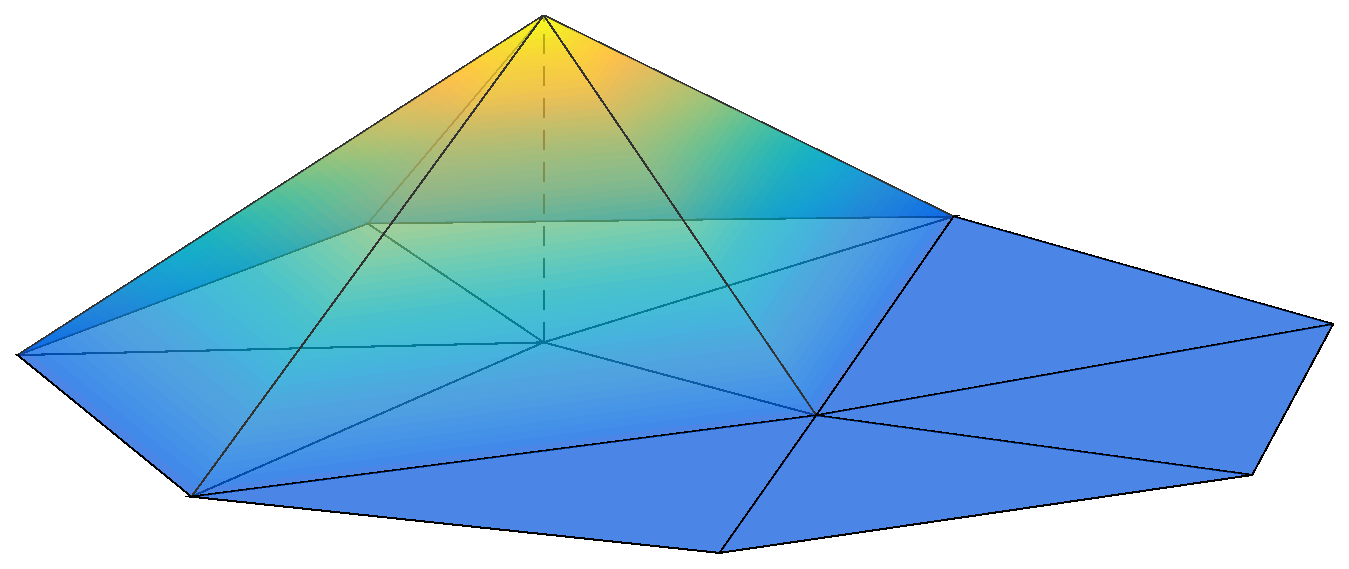
\includegraphics[width=0.48\textwidth]{shape_global_p1}
  \caption{Nodal basis $\phi_3$ for the linear finite element space $\calV_h$ defined by \eqref{eq:fe_lin_Vh}.}
  \label{fig:fe_shape_global_p1}
\end{figure}

The nodal basis, unlike many other bases, provides a convenient interpretation in the physical space.  Specifically, for $w \in \calV_h$, we have a (unique) representation
\begin{equation}
  w = \sum_{j=1}^n \hat w_j \phi_j = \sum_{j=1}^n w(z_j) \phi_j.
  \label{eq:fe_rep}
\end{equation}
We note that the coefficient $\hat w_j$ must be equal to $w(z_j)$, because $w(z_i) = \sum_{j=1}^n \hat w_j \phi_j(z_i) = \sum_{j=1}^n \hat w_j \delta_{ij} = \hat w_i$, $i = 1,\dots,n$; here, the second equality follows from the Lagrange interpolation property~\eqref{eq:fe_lagrange_basis_prop}.  In words, $\hat w_j = w(z_j)$, the value of the function $w \in \calV_h$ evaluated at the associated node $x_j$. This interpretation of nodal basis functions also allows us to readily confirm that the nodal basis is indeed a basis: for any $w \in \calV_h$, there exists a unique $\hat w \in \RR^n$ such that $w = \sum_{j=1}^n \hat w_j \phi_j$. % We can clearly express any function $w \in \calV_h$ in the form~\eqref{eq:fe_rep}; moreover the representation is unique.

We note that approximation spaces of the form~\eqref{eq:fe_lin_Vh} can be refined to yield a sequence of approximation spaces. A space $\calV_{h'}$ is said to be a \emph{refinement} of a space $\calV_h$ if
\begin{equation*}
  \calV_h \subset \calV_{h'};
\end{equation*}
i.e., every member of $\calV_h$ is also a member of $\calV_{h'}$. For a piecewise linear space, a refinement results from splitting some or all of elements in the triangulation.  Through a successive refinement of elements, we can construct a sequence of approximation spaces
\begin{equation*}
  \calV_{h_1} \subset \calV_{h_2} \subset \cdots \subset \calV_{h_n}
\end{equation*}
for $h_1 > h_2 > \dots > h_n$. (We recall that the subscript $h$ of $\calV_h$ indicates the diameter of the largest element, $h \equiv \max_{K \in \calT_h} \text{diam}(K)$.)  The ability to refine, and hence construct a sequence of enriched spaces, is important. Intuitively, we might relate this ability to arbitrary refine the approximation spaces with the ability to find an approximation that is arbitrary close to the exact solution.  We will make this notion of convergence more formal in a later lecture.

\section{Approximation spaces: essential boundary conditions}
We recall from Lecture~\ref{ch:var_form} that Dirichlet boundary conditions are treated as essential boundary conditions in the weak formulation of second-order elliptic PDEs.  The essential boundary conditions are explicitly imposed through the choice of the space.  For instance, given a mixed Poisson problem on $\Omega \subset \RR^d$ with a homogeneous Dirichlet boundary $\Gamma_D \subset \partial \Omega$, the appropriate function space is
\begin{equation*}
  \calV \equiv \{ v \in H^1(\Omega) \ | \ v|_{\Gamma_D} = 0 \}.
\end{equation*}
We wish to construct an approximation space $\calV_h \subset \calV$.

To facilitate our discussion, we first introduce a piecewise linear approximation space for $H^1(\Omega)$ (without the essential boundary condition),
\begin{equation*}
  H^1_h(\Omega) \equiv \{ v \in H^1(\Omega) \ | \ v|_K \in \PP^1(K), \ \forall K \in \calT_h \};
\end{equation*}
we note that the notation $H^1_h(\Omega)$ is \emph{not} standard in literature, but we adhere to it as it is convenient. We then introduce a piecewise linear approximation for $\calV \subset H^1(\Omega)$ with the essential boundary condition,
\begin{equation*}
  \calV_h \equiv \{ v \in \calV \ | \ v|_K \in \PP^1(K), \ \forall K \in \calT_h \};
\end{equation*}
functions in the approximation space $\calV_h$ must vanish on $\Gamma_D$ so that $\calV_h \subset \calV$.  The space $\calV_h$ is a subspace of $\calV$ because the functions restricted to element $K$ is in $\PP^1(K)$.  The space $\calV_h$ is also a subspace of $H^1_h(\Omega)$ because, while both spaces comprise piecewise linear functions, the functions in $\calV_h$ must vanish on the boundary $\Gamma_D$.

For a piecewise linear function $v \in H^1_h(\Omega)$, a condition equivalent to $v|_{\Gamma_D} = 0$ is
\begin{equation*}
  v_h(z_j) = 0 \quad \text{for all nodes $z_j$ on $\bar \Gamma_D$,}
\end{equation*}
where $\bar \Gamma_D$ is the closure of the Dirichlet boundary. 
We consider the closure so that the nodes at the boundary (i.e., endpoints in $\RR^2$) are included in the set. In other words,
\begin{equation*}
  \calV_h = \{ v \in H^1_h(\Omega) \ | \ v(z_j) = 0, \ \forall z_j \text{ on } \bar \Gamma_D \}.
\end{equation*}
For instance, in Figure~\ref{fig:fe_mesh_p1_bnd}, the piecewise linear function must vanish on the nodes $z_4$, $z_7$, $z_8$, and $z_9$.
\begin{figure}
  \centering
  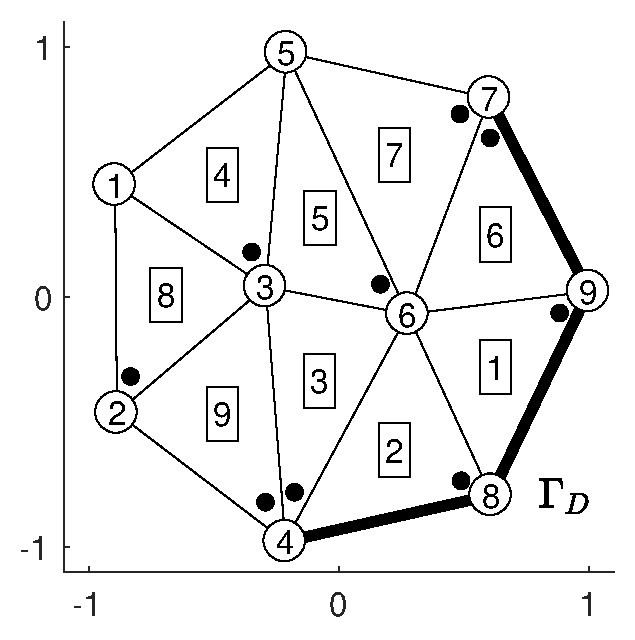
\includegraphics[width=0.35\textwidth]{fe_mesh_p1_bnd}
  \caption{A triangulated domain with a Dirichlet boundary.}
  \label{fig:fe_mesh_p1_bnd}
\end{figure}


For a nodal basis, the boundary condition can be explicitly imposed by eliminating the shape functions associated with the nodes on $\overline \Gamma_D$ from the approximation space. The dimension of the resulting approximation space for $\calV \subset H^1(\Omega)$ is
\begin{equation*}
  n \equiv \text{dim}(\calV_h) = \text{dim}(H^1_h(\Omega)) - (\text{number of nodes on $\bar \Gamma_D$}).
\end{equation*}
For instance, the dimension of the piecewise linear approximation space shown in Figure~\ref{fig:fe_mesh_p1_bnd} is $n = 9 - 4 = 5$, where the active shape functions are associated with the nodes $z_1$, $z_2$, $z_3$, $z_5$, and $z_6$. Once the set of active shape functions of $H^1_h(\Omega)$ are identified, we can readily reassign them as a basis $\{ \phi_j \}_{j=1}^n$ of $\calV_h$. Without loss of generality, we also reassign the associated node numbers $\{z_j\}_{j=1}^n$. Then, as before, we can express any function in $w \in \calV_h$ in terms of $\hat w \in \RR^n$ as
\begin{equation*}
  w = \sum_{j=1}^{n} \hat w_j \phi_j = \sum_{j=1}^{n} w(z_j) \phi_j.
\end{equation*}

We now consider an inhomogeneous Dirichlet boundary condition, say $u|_{\Gamma_D} = u^B$. We recall that the appropriate test space for the problem is $\calV \equiv \{ v \in H^1(\Omega) \ | \ v|_{\Gamma_D} = 0 \}$ and the trial space is $\calV^E \equiv u^E + \calV$, where $u^E$ is an arbitrary member of $H^1(\Omega)$ that satisfies the boundary condition $u^E|_{\Gamma_D} = u^B$.  If the boundary function $u^B$ is a piecewise polynomial that conforms to the triangulation, then it is possible to find $u^E_h \in H^1_h(\Omega)$ that satisfies the boundary condition exactly: $u^E_h|_{\Gamma_D} = u^B$.  Otherwise, we have to choose $u^E_h \in H^1_h(\Omega)$ in the piecewise polynomial space that approximately satisfies the boundary condition: $u^E_h|_{\Gamma_D} \approx u^B$.  In either case, a convenient choice (though not the only choice) is to simply choose any $u^E_h \in H^1_h(\Omega)$ such that
\begin{equation*}
  u^E_h(z_j) = u^B(z_j) \quad \text{for all nodes } z_j \text{ on } \bar \Gamma_D.
\end{equation*}
We can then express any function in $w \in \calV_h^E \equiv u_h^E + \calV_h$ in terms of $\hat w \in \RR^n$ as
\begin{equation*}
  w = u^E_h + \sum_{j=1}^n \hat w_j \phi_j,
\end{equation*}
where $\{\phi_j\}_{j=1}^n$ is a nodal basis associated with nodes not on $\bar \Gamma_D$.


%We also recall that we can reformulate the problem as follows: find $\tilde u \in \calV$ such that
%\begin{equation*}
%  a(\tilde u, v) = \tilde \ell(v) \equiv \ell(v) - a(u^E,v) \quad \forall v \in \calV,
%\end{equation*}
%and set $u = u^E + \tilde u$.  

%We now consider the construction of an approximation space for an affine space of the form
%\begin{equation*}
%  \calV^E \equiv u^E + \calV,
%\end{equation*}
%where $u^E$ is an arbitrary member in $H^1(\Omega)$ that satisfies the boundary condition $u^E|_{\Gamma_D} = u^B$.  In general, 
%\begin{equation*}
%  w = u^E_h + \sum_{j=1}^n \hat w_j \phi_j
%\end{equation*}
  


\section{Galerkin method}
We now consider a \emph{Galerkin finite element approximation} of a boundary value problem.  We first recall the weak formulation for the exact problem: find $u \in \calV$ such that
\begin{equation}
  a(u,v) = \ell(v) \quad \forall v \in \calV,
  \label{eq:fe_form_true}
\end{equation}
where $a: \calV \times \calV \to \RR$ is a coercive, continuous bilinear form and $\ell: \calV \to \RR$ is a continuous linear form.  (In general, the bilinear form needs not be coercive; however, here we assume coercivity to prove some theoretical results using the tools introduced in the previous lecture.) We now seek an approximation to~\eqref{eq:fe_form_true} in a finite-dimensional subspace $\calV_h \subset \calV$: find $u_h \in \calV_h$ such that
\begin{equation}
  a(u_h,v) = \ell(v) \quad \forall v \in \calV_h.
  \label{eq:fe_form_gal_0}
\end{equation}
This is the Galerkin finite element approximation of~\eqref{eq:fe_form_true}. In words, we obtain the finite element problem by simply restricting the test and trials spaces from $\calV$ to $\calV_h \subset \calV$.  Because the trial and test approximation spaces are the same, the method is referred to as a \emph{Galerkin method}, or, more explicitly, \emph{Bubnov-Galerkin method}.  (If the test and trial approximation spaces are different, the method is referred to as a \emph{Petrov-Galerkin method}.) The finite element problem~\eqref{eq:fe_form_gal_0} depends on the space $\calV_h$ but is independent of the particular basis $\{ \phi_i \}_{i=1}^n$ for $\calV_h$.  We will prove in Section~\ref{sec:fe_form_gal_wellposed} that the solution to~\eqref{eq:fe_form_gal_0} exists and is unique.

We now wish to recast the finite element problem~\eqref{eq:fe_form_gal_0} in linear algebraic from that is amenable to computer implementation.  To this end, we represent the solution and test functions in terms of their basis coefficients, $u_h = \sum_{j=1}^n \hat u_{h,j} \phi_j$ and $v = \sum_{i=1}^n \hat v \phi_i$ to yield the following equivalent problem for the coefficients: find $\hat u_h \in \RR^n$ such that
\begin{equation*}
  a(\sum_{j=1}^n \hat u_{h,j} \phi_j, \sum_{i=1}^n \hat v_i \phi_i)
  = \ell(\sum_{i=1}^n \hat v_i \phi_i) \quad \forall \hat v \in \RR^n.
\end{equation*}
We then invoke the bilinearity of $a(\cdot,\cdot)$ and the linearity of $\ell(\cdot)$ to obtain
\begin{equation*}
  \sum_{i,j = 1}^n \hat v_i a(\phi_j,\phi_i) \hat u_{h,j} = \sum_{i=1}^n \hat v_i \ell(\phi_i).
\end{equation*}
The problem can be more compactly expressed using the matrix-vector notation: find $\hat u_h \in \RR^n$ such that
\begin{equation}
  \hat v^T \hat A_h \hat u_h = \hat v^T \hat f_h \quad \forall \hat v \in \RR^n,
  \label{eq:fe_form_gal_3}
\end{equation}
where the \emph{stiffness matrix} $\hat A_h \in \RR^{n \times n}$ is given by
\begin{equation*}
  \hat A_{h,ij} \equiv a(\phi_j, \phi_i), \quad i,j = 1,\dots,n,
\end{equation*}
and the \emph{load vector} $\hat f_h \in \RR^n$ is given by
\begin{equation*}
  \hat f_{h,i} \equiv \ell(\phi_i), \quad i = 1,\dots,n.
\end{equation*}
In order for~\eqref{eq:fe_form_gal_3} to hold, each row of $A_h \hat u_h - f_h$ must be equal to zero; otherwise, we can find $\hat v \in \RR^n$ that is finite only on that non-zero and hence~\eqref{eq:fe_form_gal_3} would not hold.  We hence conclude that the statement \eqref{eq:fe_form_gal_3} is equivalent to finding $\hat u_h \in \RR^n$ that satisfies 
\begin{equation}
  \hat A_h \hat u_h = \hat f_h  \quad \text{(in $\RR^n$)}.
  \label{eq:fe_form_gal_4}
\end{equation}
We will prove in Section~\ref{sec:fe_form_gal_wellposed} that~\eqref{eq:fe_form_gal_4} has a unique solution.

\section{Well-posedness of the Galerkin finite element formulation}
\label{sec:fe_form_gal_wellposed}
The following proposition shows that the solution to~\eqref{eq:fe_form_gal_0} exists and is unique.
\begin{proposition}
  \label{prop:fe_form_gal_wellposed}
    Given an approximation space $\calV_h \subset \calV$, a continuous, coercive (but not necessarily symmetric) bilinear form $a: \calV \times \calV \to \RR$, and a continuous linear functional $\ell \in \calV'$, there exists a unique $u_h \in \calV_h$ such that
  \begin{equation*}
    a(u_h,v) = \ell(v) \quad \forall v \in \calV_h.
  \end{equation*}
  \begin{proof}
We will appeal to the Lax-Milgram theorem, Theorem~\ref{thm:lax_milgram}; to do so, we need to demonstrate that (i) the bilinear form $a(\cdot,\cdot)$ is coercive in $\calV_h$, (ii) the bilinear form is continuous $a(\cdot,\cdot)$ is continuous in $\calV_h$, and (iii) the linear form $\ell(\cdot)$ is continuous in $\calV_h$.  All of these properties follow from the fact that $\calV_h$ is a subspace of $\calV$.  The coercivity of $a(\cdot,\cdot)$ in $\calV_h$ follows from
\begin{equation*}
  \alpha_h \equiv \inf_{v \in \calV_h} \frac{a(v,v)}{\| v \|^2_\calV} \geq
  \inf_{v \in \calV} \frac{a(v,v)}{\| v \|^2_\calV} \equiv \alpha > 0,
\end{equation*}
where the inequality follows from $\calV_h \subset \calV$.  The coercivity constant associated with $\calV_h$, $\alpha_h$, is bounded from the below by the coercivity constant associated with $\calV$, $\alpha$, which itself is bounded from the below by $0$. The continuity of $a(\cdot,\cdot)$ in $\calV_h$ follows from
\begin{equation*}
  \gamma_h \equiv \sup_{w,v \in \calV_h} \frac{a(w,v)}{\|w\|_\calV\| v \|_\calV} \leq
  \sup_{w,v \in \calV} \frac{a(w,v)}{\| w \|_\calV\| v \|_\calV} \equiv \gamma < \infty,
\end{equation*}
where the inequality again follows from $\calV_h \subset \calV$.  The continuity constant associated with $\calV_h$, $\gamma_h$, is bounded from the above by the continuity constant associated with $\calV$, $\gamma$, which itself is finite.  Similarly, the continuity of $\ell(\cdot)$ in $\calV_h$ follows from
\begin{equation*}
  \| \ell \|_{(\calV_h)'} \equiv \sup_{v \in \calV_h} \frac{\ell(v)}{\| v \|_\calV} \leq \sup_{v \in \calV} \frac{\ell(v)}{\| v \|_\calV} \equiv \| \ell \|_{\calV'} < \infty,
\end{equation*}
where the inequality again follows from $\calV_h \subset \calV$.  Because the bilinear from is coercive and continuous in $\calV_h$ and the linear from is continuous in $\calV_h$, we conclude by the Lax-Milgram theorem that the solution exists and is unique.
  \end{proof}
\end{proposition}
Proposition~\ref{prop:fe_form_gal_wellposed} shows the existence of a unique solution to the finite element problem~\eqref{eq:fe_form_gal_0} without appealing to any specific basis for $\calV_h$; the finite element solution $u_h \in \calV_h$ depends only on the space $\calV_h$ and is independent of the specific basis $\{ \phi_i \}_{i=1}^n$ used to represent functions in $\calV_h$.

For a problem that involves inhomogeneous Dirichlet data, the well-posedness of the finite element problem can be proved using the same technique used for the exact (infinite-dimensional) problem in Section~\ref{sec:var_wellposedness}; we first reformulate it as a homogeneous Dirichlet problem with a modified linear form and then apply the Lax-Milgram theorem.

We now consider the well-posedness of the linear algebraic problem~\ref{eq:fe_form_gal_4}.
\begin{proposition}
  Under the condition of Proposition~\ref{prop:fe_form_gal_wellposed}, introduce a basis $\{\phi_i\}_{i=1}^n$ for $\calV_h$. There exists a unique solution $\hat u_h \in \RR^n$ to 
  \begin{equation*}
    \hat A_h \hat u_h = \hat f_h,
  \end{equation*}
  where $\hat A_{h,ij} \equiv a(\phi_j, \phi_i)$ and $\hat f_{h,i} \equiv \ell(\phi_i)$.
  \begin{proof}
    Proposition~\ref{prop:fe_form_gal_wellposed} shows the existence and uniqueness of the solution $\hat u_h \in \calV_h$.  Because $\{\phi_i\}_{i=1}^n$ is a basis for $\calV_h$, there exists a unique coefficients $\hat u_h \in \RR^n$ such that
    \begin{equation*}
      u_h = \sum_{j=1}^n \hat u_{h,j} \phi_j.
    \end{equation*}
    The coefficients $\hat u_h \in \RR^n$ is the unique solution of the linear system.
  \end{proof}
\end{proposition}

\emph{If} we assume that the bilinear form is not only continuous and coercive but also symmetric, then we can also show that the matrix $\hat A_h \in \RR^{n \times n}$ is symmetric positive definite and hence is non-singular. 
\begin{proposition}
  \label{prop:fe_form_Ah_spd}
  If the bilinear form $a: \calV \times \calV \to \RR$ is symmetric and coercive, then the stiffness matrix $\hat A_h \in \RR^{n \times n}$ is symmetric positive definite (SPD).
  \begin{proof}
    The symmetry of $\hat A_h$ follows directly from the symmetry of the bilinear form:
  \begin{equation*}
    \hat A_{h,ij} = a(\phi_j,\phi_i) = a(\phi_i,\phi_j) = \hat A_{h,ji} \quad  \forall i,j = 1, \dots, n.
  \end{equation*}
  To prove positive definiteness, we first observe that $\forall \hat v \in \RR^n$, 
\begin{equation*}
  \hat v^T \hat A_{h} \hat v
  =
  \sum_{i,j = 1}^n \hat v_i a(\phi_j, \phi_i) \hat v_j 
  = a(\sum_{j=1}^n \hat v_j \phi_j, \sum_{i=1}^n \hat v_i \phi_i)
  \geq \alpha \| \sum_{i=1}^n \hat v_i \phi_i \|^2_{\calV} \geq 0,
\end{equation*}
where the first inequality follows from the coercivity of $a(\cdot,\cdot)$ and the last equality follows from the positive definiteness of the norm $\| \cdot \|_{\calV}$. Moreover, because $\| \cdot \|_{\calV}$ is a norm, $\| \sum_{i=1}^n \hat v_i \phi_i \|_\calV = 0$ if and only if $\sum_{i=1}^n \hat v_i \phi_i = 0$.  In addition, because $\{\phi_i\}_{i=1}^n$ is a basis and in particular linearly independent, $\sum_{i=1}^n \hat v_i \phi_i = 0$ if and only if $\hat v_i = 0$, $\forall i = 1,\dots,n$. It follows that
\begin{equation*}
  \hat v^T \hat A_h \hat v = 0 \quad \text{if and only if} \quad \hat v = 0.
\end{equation*}
Hence, the matrix $\hat A_h \in \RR^{n \times n}$ is SPD.
  \end{proof}
\end{proposition}
\begin{remark}
  Because the matrix $\hat A_h \in \RR^{n \times n}$ is SPD, the matrix is non-singular, and the linear system $\hat A_h \hat u_h = \hat f_h$ has a unique solution.
\end{remark}

Before we conclude a section, we make an important remark.  A finite element solution $u_h \in \calV_h$ is a \emph{field} that approximates the solution $u \in \calV$. Because $u_h$ is a field, we can evaluate $u_h$ at any point $x \in \Omega$.  This is fundamentally different from a finite difference method, which approximates the solution at a discrete set of points, and the solution elsewhere is in general not approximated.  (Of course, we could in practice interpolate the finite difference solution, but that involves an additional approximation.)  While the coefficients $\hat u_h \in \RR^n$ is associated with the nodal value of the solution for nodal bases, this is a rather special interpretation for a nodal bases. The finite element solution field $u_h \in \calV_h$ only depends on the space $\calV_h$ and not the particular basis used to represent the functions in $\calV_h$. 

\section{Minimization formulation}
For a variational problem with a symmetric, coercive bilinear form, we can also formulate the finite element problem using a minimization formulation.  We recall that the energy functional associated with the minimization problem is $J: \calV \to \RR$ such that
\begin{equation*}
  J(w) \equiv \frac{1}{2} a(w,w) - \ell(w),
\end{equation*}
where $a: \calV \times \calV \to \RR$ is a symmetric, coercive bilinear form, and $\ell: \calV \to \RR$ is a linear form.  The solution is given by $u \in \calV$ such that
\begin{equation*}
  u = \argmin_{w \in \calV} J(w).
\end{equation*}
We recall that the minimization formulation and the variational formulation are equivalent.

The finite element approximation is given by the minimization problem over a subspace $\calV_h \subset \calV$. To this end, we introduce a basis $\{\phi_i\}_{i=1}^n$ for $\calV_h$ and evaluate the energy functional for an arbitrary $w \equiv \sum_{j=1}^n \hat w_j \phi_j$ in the space:
\begin{align*}
  J(w) =  J(\sum_{j=1}^n \hat w_j \phi_j)
  = \frac{1}{2} a (\sum_{j=1}^n \hat w_j \phi_j, \sum_{i=1}^n \hat w_i \phi_i) - \ell(\sum_{i=1}^n \hat w_i \phi_i)
  = \frac{1}{2} \sum_{i,j=1}^n \hat w_i \underbrace{ a(\phi_j,\phi_i) }_{\hat A_{h,ij}} \hat w_j - \sum_{i=1}^n \hat w_i \underbrace{ \ell(\phi_i) }_{\hat f_{h,i}};
\end{align*}
here identify the stiffness matrix $\hat A_h$ and load vector $\hat f_h$ in the expression. We can then redefine an energy functional in terms of the coefficients $\hat w \in \RR^n$ such that 
\begin{equation*}
  \hat J(\hat w) \equiv J(\sum_{j=1}^n \hat w_j \phi_j)
  = \frac{1}{2} \hat w^T \hat A_h \hat w - \hat w^T \hat f_h.
\end{equation*}
We then seek the coefficients $\hat u_h \in \RR^n$ such that
\begin{equation*}
  \hat u_h = \argmin_{\hat w \in \RR^n} \hat J(\hat w).
\end{equation*}
The sufficient condition for $\hat u_h$ to be the minimizer is that (i) the gradient is zero, $\nabla \hat J(\hat u_h) = 0$, and (ii) the Hessian of $J(\hat u_h)$ is SPD.  The condition (i) is equivalent to
\begin{equation*}
  \nabla \hat J(\hat u_h) = \hat A_h \hat u_h - \hat f_h = 0 \quad (\text{in } \RR^n),
\end{equation*}
which is the same as the Galerkin finite element statement for the coefficients,~\ref{eq:fe_form_gal_4}.  The condition (ii) is also satisfied because the Hessian of $J(\hat u_h)$ is $\hat A_h$, which we have proven is SPD for a symmetric, coercive bilinear form in Proposition~\eqref{prop:fe_form_Ah_spd}. Hence, the finite element solution $u_h \in \calV_h$, and the associated coefficients $\hat u_h \in \RR^n$, can also be obtained using the minimization formulation.

\section{Generalization: higher-order and spectral methods}
In this lecture, we constructed the Galerkin approximation based on an approximation space $\calV_h$ of piecewise linear ($\PP^1$) polynomials; however, the Galerkin method --- which approximates the solution $u \in \calV$ in a subspace $\calV_h$ --- is in fact a general procedure that works with any approximation space $\calV_h \subset \calV$.

For instance, we could consider a domain with a curved boundary and an associated triangulation as shown in Figure~\ref{fig:fe_form_mesh_p2}, and then considered a space of piecewise quadratic ($\PP^2$) polynomials,
\begin{equation}
  \calV_h \equiv \{ v \in \calV \ | \ v|_K \in \PP^2, \ \forall K \in \calT_h \}.
  \label{eq:fe_form_Vh_p2}
\end{equation}
An example of a function that belongs to the space is shown in Figure~\ref{fig:fe_fun_p2}.  We may compare the piecewise linear and quadratic functions shown in Figures~\ref{fig:fe_fun_p1} and \ref{fig:fe_fun_p2}, respectively, and intuitively draw a conclusion that the $\PP^2$ space provides a better approximation of smooth functions.  This intuition is in fact true; we will make mathematical argument in a later lecture. Like the $\PP^1$ space, the $\PP^2$ space can be refined by splitting some or all of elements such that $\calV_h \subset \calV_{h'}$. A successive refinements yield a sequence of approximation spaces $\calV_{h_1} \subset \calV_{h_2} \subset \dots \subset \calV_{h_n}$ for $h_1 > h_2 > \cdots > h_n$. In fact, a finite element approximations based on piecewise polynomial spaces of degree greater than 1, which include the $\PP^2$ space, are often referred to as a \emph{higher-order approximation}, because the solution converges more rapidly with $h$ than for the $\PP^1$ space. 

\begin{figure}
  \centering
  \subfigure[triangulation]{
    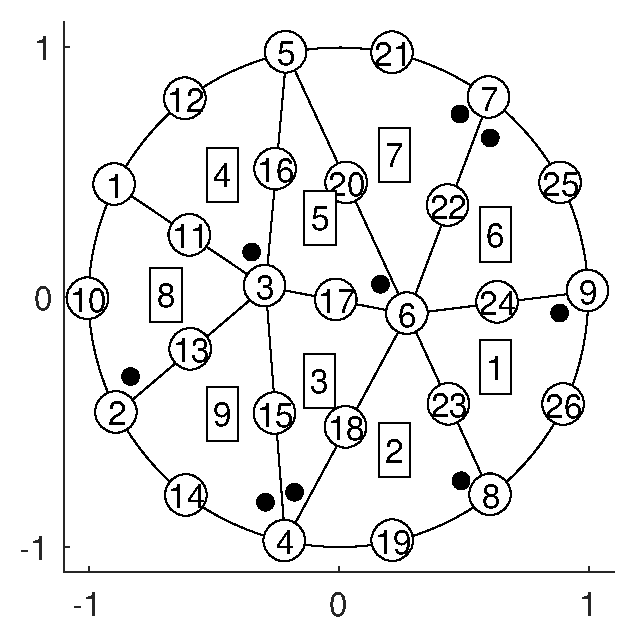
\includegraphics[width=0.3\textwidth]{fe_mesh_p2}
    \label{fig:fe_form_mesh_p2}
  }
  \subfigure[example function]{
    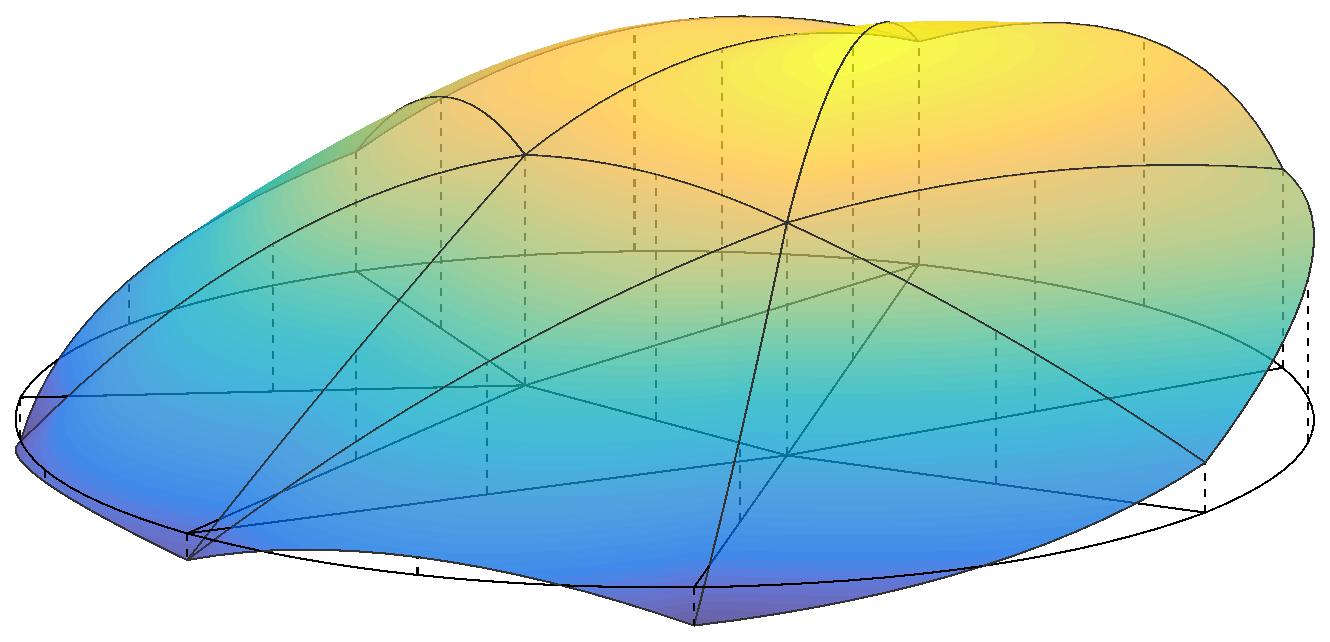
\includegraphics[width=0.4\textwidth]{fe_fun_p2}
    \label{fig:fe_fun_p2}
  }
  \subfigure[vertex shape function $\phi_3$]{
    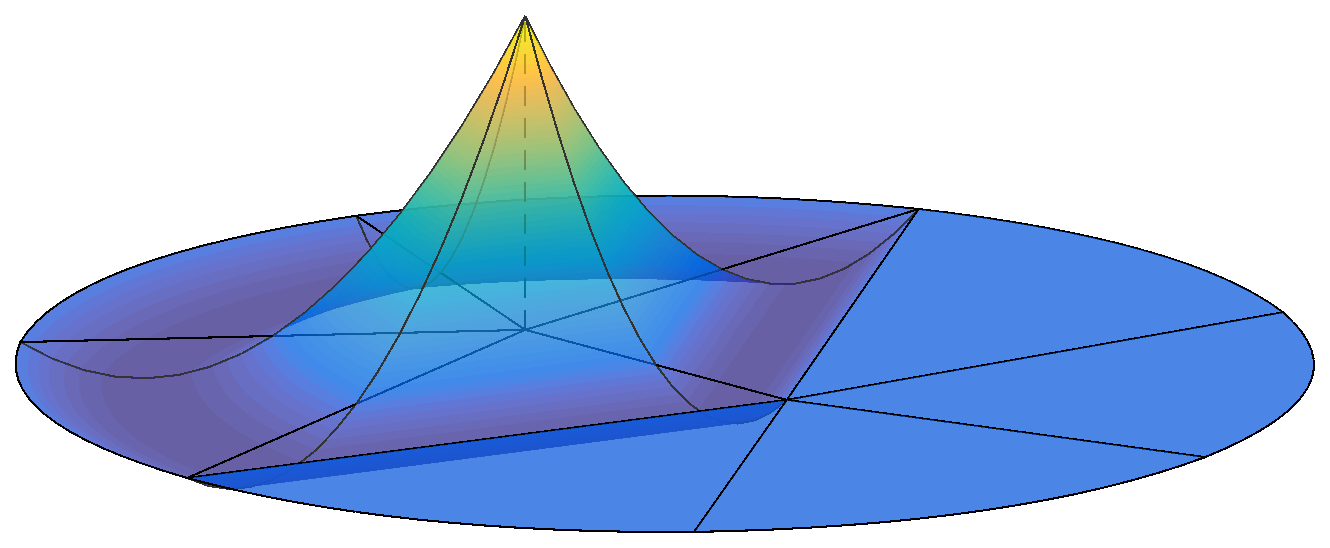
\includegraphics[width=0.4\textwidth]{shape_global_p2_1}
    \label{fig:fe_shape_global_p2_1}
  }
  \subfigure[edge shape function $\phi_{20}$]{
    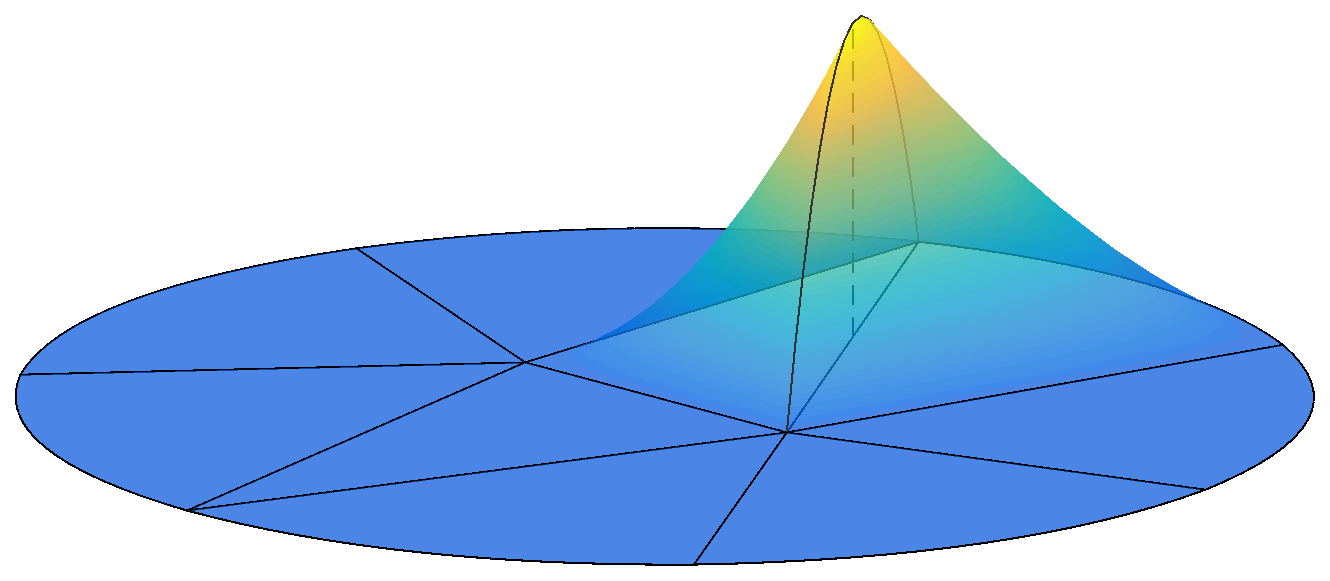
\includegraphics[width=0.4\textwidth]{shape_global_p2_2}
    \label{fig:fe_shape_global_p2_2}
  }
  \caption{$\PP^2$ finite element space.}
\end{figure}

Figures~\ref{fig:fe_shape_global_p2_1} and \ref{fig:fe_shape_global_p2_2} show two of the nodal shape functions for the $\PP^2$ space associated with the triangulation~\ref{fig:fe_form_mesh_p2}.  Unlike the nodal shape functions for the $\PP^1$ space which are associated with only vertices of the triangles, the nodal shape functions for the $\PP^2$ space are associated with either vertices or edges.  

As another example, suppose the domain of interest $\Omega$ is a line in $\RR^1$, a square in $\RR^2$, a cube in $\RR^3$, or any shape that can be mapped to these shapes. Then we can also consider an approximation space consists of global polynomials
\begin{equation*}
  \calV_p \equiv \{ v \in \calV \ | \ v \in (\PP^p(\Omega))^d \}.
\end{equation*}
In this case, the approximation space can be refined by increasing the polynomial degree; we readily observe that $\calV_{p} \subset \calV_{p'}$ for $p \leq p'$. The Galerkin finite element method based on a sequence of global polynomial spaces, $\calV_{p_1} \subset \calV_{p_2} \subset \cdots \subset \calV_{p_n}$ for $p_1 \leq p_2 \leq \cdots \leq p_n$, is called the \emph{spectral method}.  The polynomials used in the spectral methods are of very high degree; polynomial spaces of degrees of 100 and higher are routinely used.

\section{Summary}
We summarize key points of this lecture:
\begin{enumerate}
\item A triangulation $\calT_h$ is a collection of non-overlapping elements $\{K_i\}_{i=1}^{n_e}$ that covers the domain $\Omega$.
\item The act of constructing a triangulation for a given domain is called mesh generation. Mesh generation is a non-trivial task, but there are many open-source and commercial meshers.
\item An approximation space $\calV_h$ is a finite-dimensional subspace of $\calV \subset H^1(\Omega)$; the space comprises, for example, piecewise polynomials associated with the triangulation.
\item Given a basis $\{ \phi_i \}_{i=1}^n$ for $\calV_h$, any function $v \in \calV_h$ can be identified with a unique coefficients $\hat v \in \RR^n$, which are the global degrees of freedom of $\calV_h$.
\item An approximation space can be successively refined to yield a sequence of approximation spaces.
\item If a nodal basis is used for $H^1_h(\Omega)$, then a subspace $\calV_h \subset H^1_h(\Omega)$ that satisfies the essential boundary conditions can be formed by removing nodal shape functions on the closure of the Dirichlet boundary.
\item The Galerkin finite element method solves the variational problem in a finite-dimensional approximation space $\calV_h \subset \calV$.
\item Given a basis $\{\phi_i\}_{i=1}^n$ of $\calV_h$, the coefficients $\hat u_h \in \RR^n$ associated with the solution $u_h \in \calV_h$ solves a $n \times n$ linear system $\hat A_h \hat u_h = \hat f_h$, where $A_{h,ij} = a(\phi_j,\phi_i)$ and $f_{h,i} = \ell(\phi_i)$.
\item If the bilinear form is coercive and continuous and the linear form is continuous, the solution to the Galerkin finite element problem exists and is unique.
\item If the bilinear form is symmetric, coercive, and continuous, then the finite element solution $u_h \in \calV_h$ can also be obtained from the minimization principle.
\item The Galerkin finite element procedure can accommodate as its approximation space, for instance, piecewise higher-order polynomials (i.e., higher-order method) or high-order global polynomials (i.e., spectral method).
\end{enumerate}
